\section{Results and Discussion}

\begin{figure}
    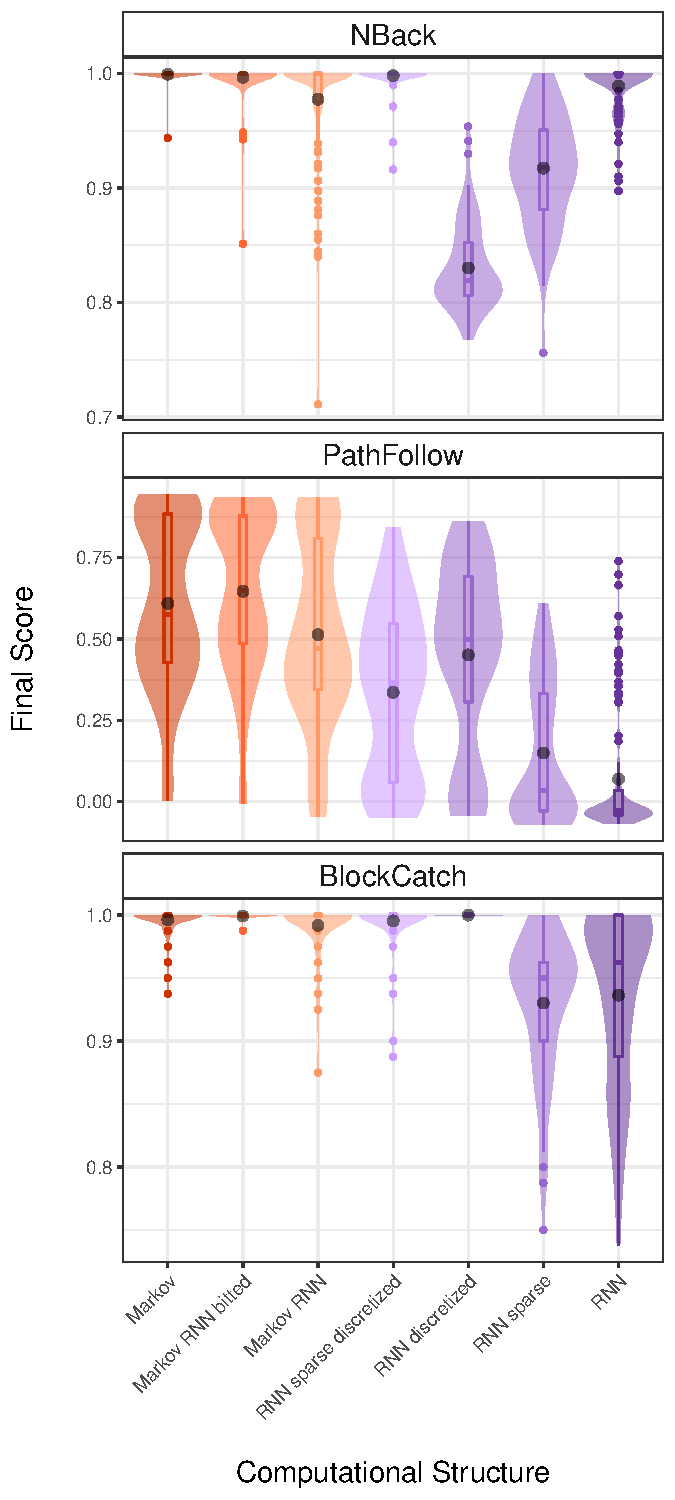
\includegraphics[width=0.45\textwidth]{chapters/2-comp-hybrid/figs/merged_LOD_data_end_score.pdf}
    \caption{Performance of computational structures across tasks. Color hue indicates the brain variant used; color saturation indicates distance in number of changes from canonical structures, with more distant hybrids being less saturated. Note the varied scales on the y-axis, as we are interested here only in comparative performance within worlds rather than across worlds.}
    \label{fig:scores}
\end{figure}

\begin{table}
% Please add the following required packages to your document preamble:
% \usepackage{graphicx}
% \usepackage[table,xcdraw]{xcolor}
% If you use beamer only pass "xcolor=table" option, i.e. \documentclass[xcolor=table]{beamer}
\begin{center}
    \textbf{Significance:} NBack
\end{center}
\resizebox{0.5\textwidth}{!}{%
\begin{tabular}{l|c|c|c|
>{\columncolor[HTML]{B3E9B4}}c |c|c|}
\cline{2-7}
\multicolumn{1}{c|}{\textbf{A}}                      & \cellcolor[HTML]{EFEFEF}\begin{tabular}[c]{@{}c@{}}Markov \\ RNN bitted\end{tabular} & \cellcolor[HTML]{EFEFEF}\begin{tabular}[c]{@{}c@{}}Markov \\ RNN\end{tabular} & \cellcolor[HTML]{EFEFEF}\begin{tabular}[c]{@{}c@{}}RNN \\ sparse/\\ discretized\end{tabular} & \cellcolor[HTML]{EFEFEF}\begin{tabular}[c]{@{}c@{}}RNN \\ discretized\end{tabular} & \cellcolor[HTML]{EFEFEF}\begin{tabular}[c]{@{}c@{}}RNN\\ sparse\end{tabular}           & \cellcolor[HTML]{EFEFEF}RNN                                                            \\ \hline
\multicolumn{1}{|l|}{\cellcolor[HTML]{EFEFEF}Markov} & 1.000                                                                                & 0.943                                                                         & 1.000                                                                                        & \begin{tabular}[c]{@{}c@{}}***\\ \textless{}0.001\end{tabular}                     & \cellcolor[HTML]{B3E9B4}\begin{tabular}[c]{@{}c@{}}***\\ 0.002\end{tabular}            & 0.999                                                                                  \\ \hline
\multicolumn{2}{|l|}{\cellcolor[HTML]{EFEFEF}Markov RNN bitted}                                                                             & 0.971                                                                         & 1.000                                                                                        & \begin{tabular}[c]{@{}c@{}}***\\ \textless{}0.001\end{tabular}                     & \cellcolor[HTML]{B3E9B4}\begin{tabular}[c]{@{}c@{}}***\\ 0.003\end{tabular}            & 1.000                                                                                  \\ \hline
\multicolumn{3}{|l|}{\cellcolor[HTML]{EFEFEF}Markov RNN}                                                                                                                                                                    & 0.957                                                                                        & \begin{tabular}[c]{@{}c@{}}***\\ \textless{}0.001\end{tabular}                     & 0.06                                                                                   & 0.998                                                                                  \\ \hline
\multicolumn{4}{|l|}{\cellcolor[HTML]{EFEFEF}RNN sparse/discretized}                                                                                                                                                                                                                                                       & \begin{tabular}[c]{@{}c@{}}***\\ \textless{}0.001\end{tabular}                     & \cellcolor[HTML]{B3E9B4}\begin{tabular}[c]{@{}c@{}}**\\ 0.002\end{tabular}            & 1.000                                                                                  \\ \hline
\multicolumn{5}{|l|}{\cellcolor[HTML]{EFEFEF}RNN discretized}                                                                                                                                                                                                                                                                                                                                                   & \cellcolor[HTML]{B3E9B4}\begin{tabular}[c]{@{}c@{}}***\\ \textless{}0.001\end{tabular} & \cellcolor[HTML]{B3E9B4}\begin{tabular}[c]{@{}c@{}}***\\ \textless{}0.001\end{tabular} \\ \hline
\multicolumn{6}{|l|}{\cellcolor[HTML]{EFEFEF}RNN sparse}                                                                                                                                                                                                                                                                                                                                                                                                                                                 & \cellcolor[HTML]{B3E9B4}\begin{tabular}[c]{@{}c@{}}**\\ 0.01\end{tabular}              \\ \hline
\end{tabular}%
}
\bigskip
% Please add the following required packages to your document preamble:
% \usepackage{graphicx}
% \usepackage[table,xcdraw]{xcolor}
% If you use beamer only pass "xcolor=table" option, i.e. \documentclass[xcolor=table]{beamer}
\begin{center}
    \textbf{Significance:} PathFollow
\end{center}
\resizebox{0.5\textwidth}{!}{%
\begin{tabular}{l|c|
>{\columncolor[HTML]{EFEFEF}}c |
>{\columncolor[HTML]{EFEFEF}}c |
>{\columncolor[HTML]{B3E9B4}}c |
>{\columncolor[HTML]{B3E9B4}}c |
>{\columncolor[HTML]{B3E9B4}}c |}
\cline{2-7}
\multicolumn{1}{c|}{\textbf{B}}                      & \cellcolor[HTML]{EFEFEF}\begin{tabular}[c]{@{}c@{}}Markov \\ RNN bitted\end{tabular} & \begin{tabular}[c]{@{}c@{}}Markov \\ RNN\end{tabular}                                  & \begin{tabular}[c]{@{}c@{}}RNN \\ sparse/\\ discretized\end{tabular}                   & \cellcolor[HTML]{EFEFEF}\begin{tabular}[c]{@{}c@{}}RNN \\ discretized\end{tabular} & \cellcolor[HTML]{EFEFEF}\begin{tabular}[c]{@{}c@{}}RNN\\ sparse\end{tabular} & \cellcolor[HTML]{EFEFEF}RNN                                    \\ \hline
\multicolumn{1}{|l|}{\cellcolor[HTML]{EFEFEF}Markov} & 0.557                                                                                & \cellcolor[HTML]{B3E9B4}\begin{tabular}[c]{@{}c@{}}***\\ \textless{}0.001\end{tabular} & \cellcolor[HTML]{B3E9B4}\begin{tabular}[c]{@{}c@{}}***\\ \textless{}0.001\end{tabular} & \begin{tabular}[c]{@{}c@{}}***\\ \textless{}0.001\end{tabular}                     & \begin{tabular}[c]{@{}c@{}}***\\ \textless{}0.001\end{tabular}               & \begin{tabular}[c]{@{}c@{}}***\\ \textless{}0.001\end{tabular} \\ \hline
\multicolumn{2}{|l|}{\cellcolor[HTML]{EFEFEF}Markov RNN bitted}                                                                             & \cellcolor[HTML]{B3E9B4}\begin{tabular}[c]{@{}c@{}}***\\ \textless{}0.001\end{tabular} & \cellcolor[HTML]{B3E9B4}\begin{tabular}[c]{@{}c@{}}***\\ \textless{}0.001\end{tabular} & \begin{tabular}[c]{@{}c@{}}***\\ \textless{}0.001\end{tabular}                     & \begin{tabular}[c]{@{}c@{}}***\\ \textless{}0.001\end{tabular}               & \begin{tabular}[c]{@{}c@{}}***\\ \textless{}0.001\end{tabular} \\ \hline
\multicolumn{3}{|l|}{\cellcolor[HTML]{EFEFEF}Markov RNN}                                                                                                                                                                             & \cellcolor[HTML]{B3E9B4}\begin{tabular}[c]{@{}c@{}}***\\ \textless{}0.001\end{tabular} & \begin{tabular}[c]{@{}c@{}}*\\ 0.045\end{tabular}                                  & \begin{tabular}[c]{@{}c@{}}***\\ \textless{}0.001\end{tabular}               & \begin{tabular}[c]{@{}c@{}}***\\ \textless{}0.001\end{tabular} \\ \hline
\multicolumn{4}{|l|}{\cellcolor[HTML]{EFEFEF}RNN sparse/discretized}                                                                                                                                                                                                                                                          & \begin{tabular}[c]{@{}c@{}}***\\ \textless{}0.001\end{tabular}                     & \begin{tabular}[c]{@{}c@{}}***\\ \textless{}0.001\end{tabular}               & \begin{tabular}[c]{@{}c@{}}***\\ \textless{}0.001\end{tabular} \\ \hline
\multicolumn{5}{|l|}{\cellcolor[HTML]{EFEFEF}RNN discretized}                                                                                                                                                                                                                                                                                                                                                      & \begin{tabular}[c]{@{}c@{}}***\\ \textless{}0.001\end{tabular}               & \begin{tabular}[c]{@{}c@{}}***\\ \textless{}0.001\end{tabular}             \\ \hline
\multicolumn{6}{|l|}{\cellcolor[HTML]{EFEFEF}RNN sparse}                                                                                                                                                                                                                                                                                                                                                                                                                                          & \begin{tabular}[c]{@{}c@{}}**\\ 0.002\end{tabular}              \\ \hline
\end{tabular}%
}
\bigskip
% Please add the following required packages to your document preamble:
% \usepackage{graphicx}
% \usepackage[table,xcdraw]{xcolor}
% If you use beamer only pass "xcolor=table" option, i.e. \documentclass[xcolor=table]{beamer}
\begin{center}
    \textbf{Significance:} BlockCatch
\end{center}
\resizebox{0.5\textwidth}{!}{%
\begin{tabular}{l|c|
>{\columncolor[HTML]{EFEFEF}}c |
>{\columncolor[HTML]{EFEFEF}}c |
>{\columncolor[HTML]{FFFFFF}}c |
>{\columncolor[HTML]{B3E9B4}}c |
>{\columncolor[HTML]{FFFFFF}}c |}
\cline{2-7}
\multicolumn{1}{c|}{\textbf{C}}                      & \cellcolor[HTML]{EFEFEF}\begin{tabular}[c]{@{}c@{}}Markov \\ RNN bitted\end{tabular} & \begin{tabular}[c]{@{}c@{}}Markov \\ RNN\end{tabular} & \begin{tabular}[c]{@{}c@{}}RNN \\ sparse/\\ discretized\end{tabular} & \cellcolor[HTML]{EFEFEF}\begin{tabular}[c]{@{}c@{}}RNN \\ discretized\end{tabular} & \cellcolor[HTML]{EFEFEF}\begin{tabular}[c]{@{}c@{}}RNN\\ sparse\end{tabular} & \cellcolor[HTML]{EFEFEF}RNN \\ \hline
\multicolumn{1}{|l|}{\cellcolor[HTML]{EFEFEF}Markov} & 1.000                                                                                & \cellcolor[HTML]{FFFFFF}1.000                         & \cellcolor[HTML]{FFFFFF}1.000                                        & 1.000                                                                              & \begin{tabular}[c]{@{}c@{}}*\\ 0.029\end{tabular}                            & 0.087                       \\ \hline
\multicolumn{2}{|l|}{\cellcolor[HTML]{EFEFEF}Markov RNN bitted}                                                                             & \cellcolor[HTML]{FFFFFF}0.999                         & \cellcolor[HTML]{FFFFFF}1.000                                        & 1.000                                                                              & \begin{tabular}[c]{@{}c@{}}*\\ 0.017\end{tabular}                            & 0.057                       \\ \hline
\multicolumn{3}{|l|}{\cellcolor[HTML]{EFEFEF}Markov RNN}                                                                                                                                            & \cellcolor[HTML]{FFFFFF}1.000                                        & 1.000                                                                              & \cellcolor[HTML]{FFFFFF}0.055                                                                      & 0.146                       \\ \hline
\multicolumn{4}{|l|}{\cellcolor[HTML]{EFEFEF}RNN sparse/discretized}                                                                                                                                                                                                       & 1.000                                                                              & \begin{tabular}[c]{@{}c@{}}*\\ 0.029\end{tabular}                            & 0.090                       \\ \hline
\multicolumn{5}{|l|}{\cellcolor[HTML]{EFEFEF}RNN discretized}                                                                                                                                                                                                                                                                                                   & \begin{tabular}[c]{@{}c@{}}*\\ 0.015\end{tabular}                            & 0.051                       \\ \hline
\multicolumn{6}{|l|}{\cellcolor[HTML]{EFEFEF}RNN sparse}                                                                                                                                                                                                                                                                                                                                                                                       & 1.000                       \\ \hline
\end{tabular}%
}
\bigskip 
\caption{Differences (p-value) between mean performance on tasks (A) NBack, (B) PathFollow, and (C) BlockCatch. Green cells indicate significant difference. P-values corrected using Tukey method for a family of 7 estimates. * $= p \leq 0.05$; ** $=p \leq 0.01$; *** $=p \leq 0.001$. }
\end{table}

We present here results from an application of the Comparative Hybrid Approach where we compare Markov Brains and RNNs as a demonstration of the method's qualitative analytical power. 
By identifying architectural differences between brain types and creating intermediate ``hybrids" of the two computational structures, we gain the ability to analyze how performance varied across hybrid structure and task. 
We are then able to examine whether our assumptions about the architectural differences separating the substrates map to the quantitative difference separating their performance.

\subsection{Primary Results Analysis}

We saw that Markov brains generally suffered significant performance loss when their logic lookup table gates were replaced with RNN-like threshold gates with continuous values. 
However, performance was stable or even increased when those threshold gates were used in consort with discrete memory. 
This indicates that discretization, rather than the logic lookup table structure, accounts, at least in part, for the high performance of Markov Brains on the tasks we investigated. 
The results are not as clear when we consider the RNN variants. 
While we can clearly see that the RNN variant which is both sparse \textit{and} discretized out perform canonical RNNs in all three tasks, changes in independent task performance do not clearly indicate whether it is sparsity or discretization that is the primary factor---in fact, the results indicate that the benefits conferred by each feature are task dependent.

Overall, from these results, we tentatively conclude that discretizing outputs results in generally higher performance than biasing towards network sparsity. 
However, we note that all versions of Markov Brains tend to have higher sparsity compared to all versions of RNN, and so we can not discount that sparsity plays a significant role in explaining Markov Brains' generally higher performance.

\subsection{Cross-Brain Examination: Discretization}

\subsubsection{Discretization Helps Performance on BlockCatch and PathFollow} In two of the tasks, BlockCatch and PathFollow,  discretizing the RNN memory resulted in significant performance gains, while sparsity of the network had little effect. 
In addition, the effect of combining sparsity and discretization resulted in performance that was lower than that of the RNNs that were only discretized.
In all cases, hybrid Markov Brains (i.e. with RNN gates) display higher performance when discretized (i.e. bitted) in these same tasks. 
Moreover, we were surprised to see that in PathFollow, the Markov ANN bitted hybrids outperform the canonical Markov Brains.

\subsubsection{Discretization or Sparsity Alone Hinder, But Together Help in RNN Hybrids Performance on NBack} The advantages of discretization do not carry across all types of tasks as the results from NBack attest. 
The RNN NBack results are clearly different than the other two tasks in multiple ways; we see a performance gain \textit{only} in the combined sparse-discretized network where as discretized-only and sparse-only RNN hybrids experienced performance \textit{loss}.

\subsection{Other Factors To Consider}
Based on the contradictory results observed in relation to the NBack task, we turn to the examination of other specific brain features and task details for insights that might help to explain these results. 
The following are some conjectures on possible explanations for our observed results, and should be seen as theoretical.

\subsubsection{Potential Influence of Encoding} It is possible that only considering the difference between the RNN and Markov Brain architectures is insufficient to explain the differences in performance.  
Even though both structures are built from the same type of genomes with the same mutational properties, the process which is used to map the genomes to the two types of brains is quite different. 
RNNs use a direct encoding method where a contiguous region at the beginning of the genome is read and each position in the genome relates to a particular feature in the brain (a bias or a weight). 
In contrast, Markov Brains rely on biologically inspired ``start codons" that mark coding regions. 
The RNN encoding means that the number of coding sites in the genome is constant, but because the number of start codons in a Markov Brains genome can vary, the number of coding sites can also vary. 
This results in a fixed number of effective mutations in RNNs but a variable number of effective mutations in Markov Brains. 
Because of these differences in encoding, the ways that brains are affected by mutation and the resulting evolutionary pathways may be very different. 
Further consideration of this is outside of the scope of this work, but we stress that the encoding methods could account for differences in observed performance and that future work should consider comparisons of encoding methods.

\subsection{Information Integration}

One factor that we believe could be critical to understanding these results and the results of our proposed method in general relate to the cognitive and memory requirements of the tasks being used. 
In two of the tasks, BlockCatch and PathFollow, we saw a gradient of performance across hybrids as we generally expected. 
The alterations of the RNNs caused them to perform more similarly to the Markov Brains (high performance), and the alterations of the Markov Brains caused them to perform more similarly to the RNNs (lower performance). 
However, this was not the case in the NBack task.

If we consider all three tasks from the standpoint of the cognitive abilities that each task requires, we can see that NBack only requires simple feed forward memory, while the other two tasks require long term memory and some level of information integration. 
Information integration is the ability to arrive at an answer that requires more than simple memory. 

NBack can be solved by an agent that simply stores the incoming bit string in a ``delay" buffer and delivers these stored values to the correct outputs over time. 
Each output relies only on a single prior input.

In PathFollow, agents must be able to integrate information over time. 
When the agent starts on a new path, they do not yet know which turn signal is associated with which turn. 
They must use trial and error to establish if they are in a ``$0$ means left and $1$ means right" path or a ``$1$ means left and $0$ means right" path. 
This requires that they make a guess when they arrive at the first turn signal. 
If they stay on the path then they ``know" that they guessed correctly, but if they step off the path then they must not only remember that they guessed incorrectly, but also must navigate back onto the path. 
During this process (of getting back onto the path) their sensors will not provide them with any useful input, so they must remember what part of the path recovery process they are executing. 
Finally, integration over sensors is needed. 
In order to detect a turn signal, agents must look at at least two inputs: the ``turn signal" input, and either the ``on turn" input or both the ``on forward" and ``off path inputs".

Finally, Block Catch requires that agents identify the size and direction of falling blocks. 
The identification of the left/right direction requires information integration (i.e. at least the integration of sensor states from consecutive time steps), while the identification of block size can be achieved by integration over time and sensor space or just over time.

From this it follows that the optimal logic and wiring for NBack should be simple and sparse. 
In fact there is no advantage in NBack to being able to integrate or even alter the input values. 
Arguably, a ``pass though" gate which simply moves a single value from T to T+1 should be optimal. 
It is unclear why canonical RNNs perform well on NBack versus the discretized-only and sparse-only hybrids but we conjecture that these intermediate hybrids resulted in less navigable fitness landscapes. 
 
PathFollow and Block Catch both require more complex models of memory and more complex methods of manipulating data than NBack. 
We believe that this accounts for the primary variance between the results of NBack and the results of PathFollow and Block Catch.

While this study was not designed to detect how information integration may impact optimal cognitive structures, our results indicate that such integration should be considered in future work.
